%für Sprache, A4 Blatt, float, Grafiken, UTF Codierung, PDF, Color, Seitenabstand, Listings
\documentclass[a4papr,12pt]{article}
\usepackage[utf8]{inputenc}
\usepackage[ngerman]{babel}
\usepackage{graphicx}
\usepackage{float}
\usepackage{textcomp}
\usepackage{pdfpages}
\usepackage{tikz}
\usepackage{hyperref}
\usepackage{geometry}
\usepackage{listings}
\usepackage{color}

%Mathematics
\usepackage{amstext}
\usepackage{amssymb}
\usepackage{amsmath}
\usepackage{amsfonts}
\usepackage{mathrsfs}
\usepackage{mathtools}

%include this before fancy or page style gets messed up bc of geometry
%Seitenabstand A4 Blatt
\geometry{a4paper}
\geometry{top=25mm,bottom=25mm,left=23mm,right=20mm}

% macro to select a scaled-down version of Bera Mono (for instance)
\makeatletter
\newcommand\BeraMonottfamily{%
  \def\fvm@Scale{0.85}% scales the font down
  \fontfamily{fvm}\selectfont% selects the Bera Mono font
}
\makeatother

%Hyperref zum anklicken von Überschriften in Texmaker + Farben einstellen
\hypersetup{
	colorlinks,
	citecolor=black,
	filecolor=black,
	linkcolor=blue,
	urlcolor=black
}

\definecolor{mygreen}{rgb}{0,0.6,0}
\definecolor{mygray}{rgb}{0.5,0.5,0.5}
\definecolor{mymauve}{rgb}{0.58,0,0.82}

%Zum Pascal Code einfügen mit lstinputlisting[language=Pascal] {../blabla.pas}
\lstset{ %
  backgroundcolor=\color{white},   % choose the background color; you must add \usepackage{color} or 								  \usepackage{xcolor}
  basicstyle=\BeraMonottfamily,        % the size of the fonts that are used for the code
  breakatwhitespace=false,         % sets if automatic breaks should only happen at whitespace
  breaklines=true,                 % sets automatic line breaking
  captionpos=b,                    % sets the caption-position to bottom
  commentstyle=\color{mygreen},    % comment style
  deletekeywords={...},            % if you want to delete keywords from the given language
  escapeinside={\%*}{*)},          % if you want to add LaTeX within your code
  extendedchars=true,              % lets you use non-ASCII characters; for 8-bits encodings only, 												does not work with UTF-8
  frame=single,	               % adds a frame around the code
  keepspaces=true,                 % keeps spaces in text, useful for keeping indentation of code 									  (possibly needs columns=flexible)
  keywordstyle=\color{blue},       % keyword style
  language=Octave,                 % the language of the code
  otherkeywords={...},           % if you want to add more keywords to the set
  numbers=left,                    % where to put the line-numbers; possible values are (none, left, 								  right)
  numbersep=5pt,                   % how far the line-numbers are from the code
  numberstyle=\tiny\color{black}, % the style that is used for the line-numbers
  rulecolor=\color{black},         % if not set, the frame-color may be changed on line-breaks within 								  not-black text (e.g. comments (green here))
  showspaces=false,                % show spaces everywhere adding particular underscores; it 														overrides 'showstringspaces'
  showstringspaces=false,          % underline spaces within strings only
  showtabs=false,                  % show tabs within strings adding particular underscores
  stepnumber=2,                    % the step between two line-numbers. If it's 1, each line will be 								  numbered
  stringstyle=\color{mymauve},     % string literal style
  title=\getlstname,
  tabsize=2,	                    % sets default tabsize to 2 spaces
  inputencoding=latin1,
  columns=fullflexible
}

\lstset{literate=%
	{Ö}{{\"O}}1
	{Ä}{{\"A}}1
	{Ü}{{\"U}}1
	{ß}{{\ss}}1
	{ü}{{\"u}}1
	{ä}{{\"a}}1
	{ö}{{\"o}}1
	{~}{{\textasciitilde}}1
}

%Filenamen und Pfad trennen
\makeatletter
\DeclareRobustCommand{\getlstname}{%
\begingroup
  % \lstname seems to change hyphens into \textendash
  \def\textendash{-}%
  \filename@parse{\lstname}%
  \texttt{\filename@base.\filename@ext}%
\endgroup
}


%Für Kopfzeile den Style
\usepackage{fancyhdr}
\pagestyle{fancy}
\lhead{ADE - Übung 4}
\rhead{Andreas Roither, \today{}}
\newcommand{\Cross}{\mathbin{\tikz [x=1.4ex,y=1.4ex,line width=.2ex] \draw (0,0) -- (1,1) (0,1) -- (1,0);}}%

\begin{document}

%ANGABE 
\thispagestyle{plain}
\includepdf[pages={1},pagecommand={     
\begin{tikzpicture}[remember picture, overlay]\node at (15.8, -1.35) {5 h};\end{tikzpicture}
\begin{tikzpicture}[remember picture, overlay]\node at (7.6, -1.35) {Andreas Roither};\end{tikzpicture}
\begin{Huge}
\begin{tikzpicture}[remember picture, overlay]\node at (-1.3, -1.9) {X};\end{tikzpicture}
\end{Huge}
}]{Angabe/Uebung04.pdf}
\includepdf[pages=2-,pagecommand={}]{Angabe/Uebung04.pdf}

\section*{Übung 4}
\subsection*{Aufgabe 1}
\subsubsection*{Lösungsidee}
Für das Umwandeln in andere Basen wird eine allgemeine Formel verwendet. Dazu wird ein String verwendet in dem alle erlaubten Zeichen sind, gleichzeitig wird die Position des Zeichens im String als Wertigkeit des Zeichens in der Basis 10 verwendet.

\lstinputlisting[language=Pascal] {../base2to36.pas}
\begin{figure}[H]
	\centering
	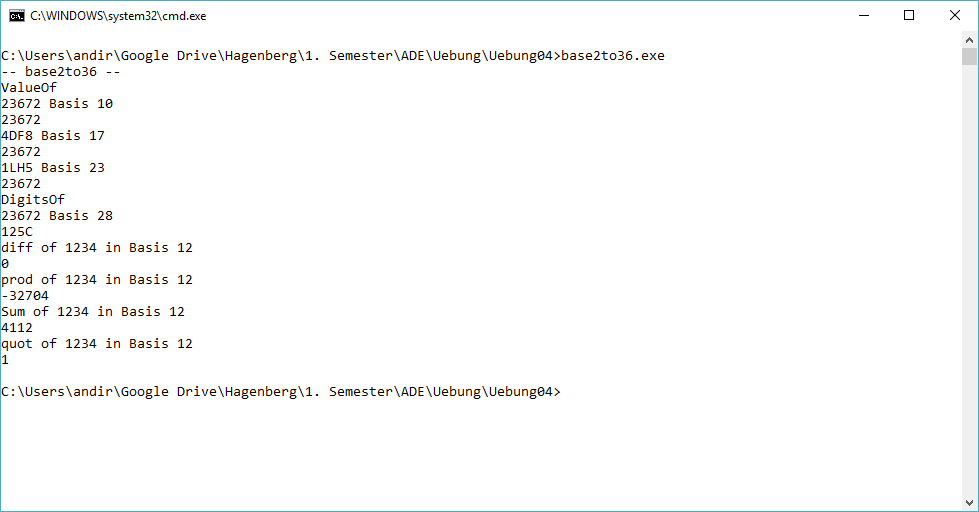
\includegraphics[scale=0.75]{./pictures/base2to36.png}
	\caption{Testfälle Basis 2 bis 36}
	\label{fig: Spannweiten Berechnung}
\end{figure}

\section*{Testfälle}
Zum Testen werden verschiedene Basen verwendet, dabei soll immer dieselbe Zahl ausgegeben werden.
Anschließend wird noch ein Zahl in der 10 Basis in der 28er Basis ausgegeben. Zum Schluss werden Diff, Sum, Prod und quot ausgegeben (mit 1234 in Basis 12), wobei bei Prod eine negative Zahl ausgegeben wird weil der Bereich überschritten wird. Dasselbe kann auch bei Sum passieren wenn zu hohe Zahlen verwendet werden.

\newpage

\subsection*{Aufgabe 2}
\subsubsection*{Lösungsidee}
Beim Balkendiagramm redone wird ein String verwendet an dem immer die jeweilige Zeile für einen Politiker angehängt und anschließend ausgegeben wird.

\lstinputlisting[language=Pascal] {../balkendiagramm_redone.pas}
\begin{figure}[H]
	\centering
	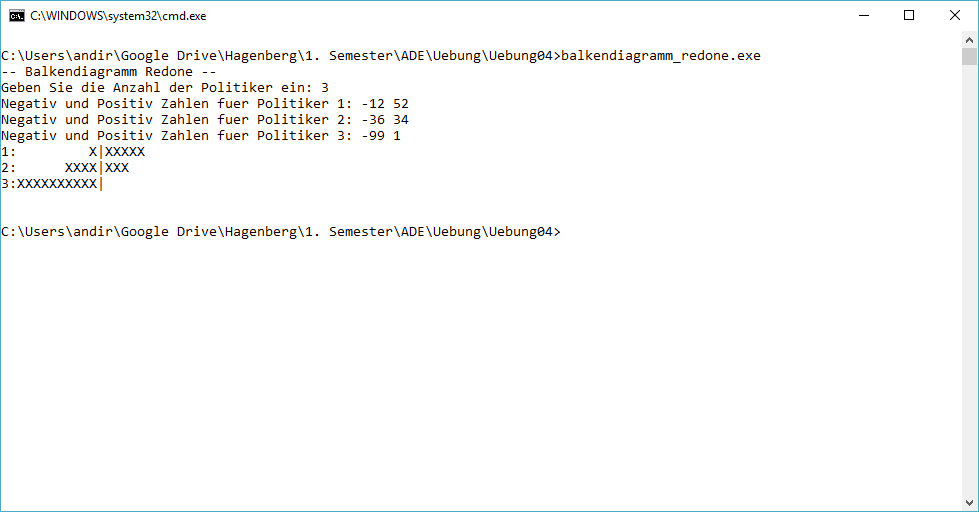
\includegraphics[scale=0.75]{./pictures/balkendiagramm_redone.png}
	\caption{Testfälle Balkendiagramm}
	\label{fig: Sortieralgorithmus}
\end{figure}

\section*{Testfälle}
Es werden drei Politiker eingegeben mit unterschiedlichen Zahlen.

\newpage

\subsection*{Aufgabe 3}
\subsubsection*{Lösungsidee}
Zum finden der fehlenden Zahl wird eine Folge von Zahlen aufsummiert und dann von einer Check Summe abgezogen. Der Rest ist das fehlende Element.

\lstinputlisting[language=Pascal] {../missingelement.pas}
\begin{figure}[H]
	\centering
	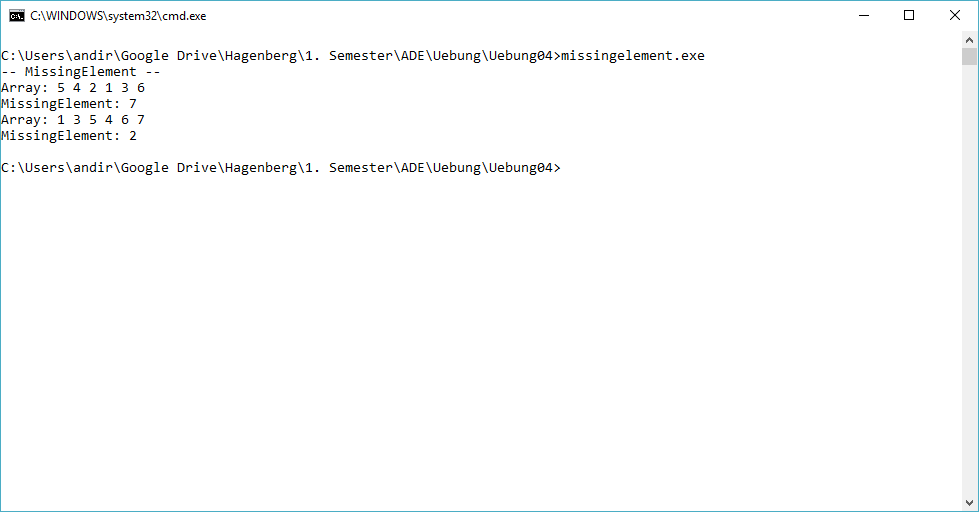
\includegraphics[scale=0.75]{./pictures/missingelement.png}
	\caption{Testfall missingelement}
	\label{fig: label}
\end{figure}

\section*{Testfall}
Ein Array mit einer Test Größe von 7 wird mit Zahlen in beliebiger Reihenfolge gefüllt und das fehlende Element wird ausgegeben. Dasselbe wird mit einem zweiten Array, mit einem anderen fehlenden Element, gemacht.

\newpage

\end{document}





